\section{Introduction}
%
Equalizers (EQs) \cite{Valimaki2016} are fundamental tools for audio signal
processing, more precisely for filtering, where spectra of audio signals
are intentionally reshaped.
%
For traditional shelving filters
\cite{Kimball1938, Zolzer2011, Reiss2015, Jot2015}, realized as infinite
impulse response (IIR) filters, cutoff frequency, shelving level and $Q$-factor
are design specifications and determine the placement of $M$ poles and $M$ zeros.
%
The steepness of the slope is typically linked to level.
%
For practical levels, a somewhat steeper or flatter slope can be
realized at the cost of frequency responses that are
underdamped (large $Q$) or overdamped (small $Q$), respectively.
%
For the mentioned filter designs of order $M$, the transition slope and bandwidth
are not independently adjustable and for large levels the slope
is always restricted to $\pm 6 \cdot M$ dB/oct, cf. \cite{Holters2006a}.
%
However, the slope and bandwidth of the transition band can be considered
as design specifications, cf. \cite{McGrath2004}.
%
Fractional-order system theory allows to design filters with arbitrary
slope $\nu$~dB/oct ($\nu\in\mathbb{R}$) \cite{Helie2013, Acharya2014}.
%
The intended accuracy of the slope determines the required IIR filter order $M$.
%
A suitable filter design determines their specific alignment.
%
By that shelving filters could be enhanced for separate adjustment of
shelving level and arbitrary slope or lower/upper cutoff frequencies
(determining the bandwidth of the slope).
%
A finite impulse response (FIR) filter design is straightforward.
%
However, standard FIR designs exhibit a linear frequency scale.
%
Thus, control of low frequencies requires a rather long impulse response and
comparably high computational complexity.
%
This might be lowered by a cascade of IIR filters with
inherent minimum phase.
%
The slope of a fractional-order filter and particular its minimum phase
characteristic is a desired property in certain audio applications
\cite{McGrath2004,Spors2010a}.
%
%
%
\NewL In \cite{Schultz2016} a cascade design of second-order shelving
filters with $\pm 3$~dB/oct slope was introduced, to
approximate the frequency response
of the so called half-differentiator/-integrator ($\pm 45$ deg minimum phase)
within certain bandwidth.
%
H{\'e}lie~\cite{Helie2013} recently introduced
a fractional-order lowpass filter design from parallel connection of poles.
%
The treatise gives the theoretical link to the so called diffusive
representation, which represents the transfer function of
a fractional-order lowpass as an integral over infinite,
infinitesimally shifted poles.
%
Approximating this integral by a finite sum leads to a parallel filter
structure.
%
This can be converted to a cascade \cite{Liski2019IEEE}.
%
The usage of a finite number of poles introduces ripples to the ideal
fractional-order slope.
%
In the present contribution, a shelving filter cascade upon this
fundamental concept is designed as generalization of \cite{Schultz2016}
towards a shelving filter with arbitrary fractional-order
slope and adjustable bandwidth.
%
The approach thus explicitly controls the transition band
and could not be traced in literature, but naturally there
are strong links to other filter design concepts.
%
These will be briefly outlined in the following.
%
%
%
\NewL Research on (digital) fractional-order filter design is particularly
pursued in control engineering, cf.
\cite{Chen2003,Barbosa2005,Barbosa2006,Tseng2017}.
%
These IIR filter designs approximate a fractional-order system and pay
special attention to the optimum slope and phase in a specified bandwidth.
%
This often comes at the cost of disregarded shelving bands, which might exhibit
arbitrary magnitude, phase and/or ripple.
%
The low-order -3~dB/oct fractional-order slope lowpass IIR filters
collected in \cite{Whittle2011} are popular in audio engineering,
e.g. to create pink from white noise.
%
%
%
\NewL Furthermore in audio, a cascade of parametric EQs (PEQs) or
shelving filters is often pursued, typically to obtain a
graphical EQ (GEQ) \cite{Holters2006b,Valimaki2017} or a
parametric multiband EQ \cite{McGrath2004,Eastty2008,Eastty2015,Lorente2017}.
%
%
In \cite{McGrath2004} adjustable fractional-order slope and bandwidth
was introduced to shelving filters for loudspeaker
controllers.
%
Using a raised-cosine slope---approximated by a PEQ cascade---%
enhanced the capabilities to equalize sound reinforcement systems.
%
Higher-order shelving slopes without excessive under-/overdamping can be
achieved by higher-order shelving filters \cite{Holters2006a}.
%
This does not allow to design the slope explicitly, but it is linked
to the level and the filter order, as stated before.
%
An example for this characteristic is depicted in
\fig{fig:holters2006-higher-order-shelving} in the present paper.
%
The design in \cite{Holters2006a} allows for
band-shelving filters with steep transition between the pass band and the
shelving band.
%
In \cite{Holters2006b} this was used to design a GEQ
with a cascade of sharp band-shelving filters.
%
With \cite{Holters2006a, Holters2006b} the multiband EQ
described in \cite{Lorente2017} can be straightforwardly designed:
%
A customized cascade is used
to realize multiple band-shelving filters, where asymmetric slopes are linked
to level and filter order.
%
Similar to \cite{McGrath2004} this design enhances capabilities for
sound reinforcement system equalization.
%
A further design \cite{Eastty2008, Eastty2015} uses
cascaded fractional-order shelving filters to obtain a shelving filter
with adjustable lower and upper cutoff frequency and corresponding levels.
%
By that a transition bandwidth is explicitly defined.
%
The slope is optimized such that an intended sharpness in the transition band
is suitable for a target application.
%
For their fractional-order shelving prototypes, the works \cite{Eastty2008, Eastty2015}
use the fact, that
a certain integer order shelving filter with a certain chosen level
yields a specific fractional-order slope in a limited bandwidth.
%
%
%
\NewL In comparison to the mentioned multiband EQs, our paper aims at shelving
filters with adjustable fractional-order slopes over a larger bandwidth,
for which the resulting minimum phase can be useful in certain applications.
%
The paper is thus organized as follows:
%
In Sec.~\ref{sec:filter_design} the filter design method and parametrization
is discussed.
%
In Sec.~\ref{sec:analog_filter_properties} the tuning and limitation properties
of the analog filter type are explained in detail.
%
In Sec.~\ref{sec:discussion} digital filter design, comparison to a digital GEQ design
and potential applications are
discussed.
%
Sec.~\ref{sec:summary} briefly summarizes the outcome.
%
All source
code\footnote{\url{https://github.com/spatialaudio/aes148-shelving-filter}}
to this paper is available.
%, supporting open science paradigms.

\section{Filter Design Method}
\label{sec:filter_design}
The analog filter design found e.g. in \cite[Sec. 3.2]{Valimaki2016},
\cite{Spors2019} is used to realize shelving filters with mid-level cutoff
frequency definition.
%
This is known as \textit{one-half-pad loss} filter characteristic
\cite{Kimball1938}. % since early days of electro-acoustics.
%
For convenience the resulting filter coefficients for 1st/2nd low-/high-shelving
filters are reviewed in the Appendix.
%
The discussion of the filter design method concentrates on the cascade of
2nd order low-shelving filters in the remainder.
%
Cascading high-shelving filters is straightforward.
%
%##############################################################################

\subsection{Cascade of 2nd Order Low-Shelving Filters}
%
The cascade (i.e. the series connection) of $N$  2nd order filters (biquads)
is given as transfer function
%
\begin{align}
\label{eq:cascade}
H(s) = \frac{Y(s)}{X(s)} = \prod\limits_{\mu=0}^{N-1} H_\mu(s)
\end{align}
in Laplace domain, being sketched in \fig{fig:tikz-cascade-biquads}.
%
The $\mu$-th biquad of the cascade is defined as, cf. \eq{eq:generalHbiquad}
%
\begin{align}
H_\mu(s) = \frac
{b_{2,\mu}\,s^2 + b_{1,\mu}\,s + b_{0,\mu}}
{a_{2,\mu}\,s^2 + a_{1,\mu}\,s + a_{0,\mu}},
\end{align}
with the corresponding coefficients, cf. \eq{eq:LS2nd}
%
\begin{align}
b_{2,\mu} = \frac{1}{\omega_{\mathrm{c},\mu}^2},\,\,\,
b_{1,\mu} = \frac{g_\mathrm{B}^{\pm\frac{1}{4}}}{Q \, \omega_{\mathrm{c},\mu}},\,\,\,
b_{0,\mu} = g_\mathrm{B}^{\pm\frac{1}{2}},\\\nonumber
a_{2,\mu} = \frac{1}{\omega_{\mathrm{c},\mu}^2},\,\,\,
a_{1,\mu} = \frac{g_\mathrm{B}^{\mp\frac{1}{4}}}{Q \, \omega_{\mathrm{c},\mu}},\,\,\,
a_{0,\mu} = g_\mathrm{B}^{\mp\frac{1}{2}},
\end{align}
%
with mid-level cutoff frequency $\omega_{\mathrm{c},\mu}$ in rad/s and
the pole/zero $Q$-factor.
%
The required gain parameter $g_\mathrm{B} = 10^{|G_\mathrm{B}|/20}>0$
is derived from the biquad shelving level $G_\mathrm{B}$ in dB.
%
The $\pm$ exponent corresponds to positive/negative $G_\mathrm{B}$.
%
The biquad shelving level $G_\mathrm{B}$ is determined by the
filter design algorithm in \eq{eq:Gb}.
%
While $G_\mathrm{B}$ and the user definable $Q$-factor are held constant for all $\mu$,
the frequency $\omega_{\mathrm{c},\mu}$ is varied over $\mu$ by the filter design
algorithm.
%
In \fig{fig:schematic_magres_2nd_ls} the level response of a single
low shelving biquad is schematically shown.
%

%

%

\definecolor{pyplotC0}{RGB}{31,119,180}
\begin{figure}[t!]
\centering
%
\begin{subfigure}{0.45\textwidth}
\centering
\documentclass{standalone}
\usepackage{tikz}

\begin{document}
\definecolor{pyplotC0}{RGB}{31,119,180}
\newcommand{\biquad}[1]{\protect\tikz[baseline=0ex]
  \protect\draw [draw=gray, very thick, scale=0.60, rounded corners=0.5mm]
  (0, 0) -- (#1, 0) -- (#1+0.25, 0.3) -- (1.25, 0.3) {};}
\newcommand{\shelf}{\protect\tikz[baseline=0ex]
  \protect\draw [ultra thick, scale=1, rounded corners=0.5mm, color=pyplotC0]
  (0, 0) -- (0.15, 0) -- (0.85, 0.6) -- (1, 0.6) {};}

\begin{plottikz}
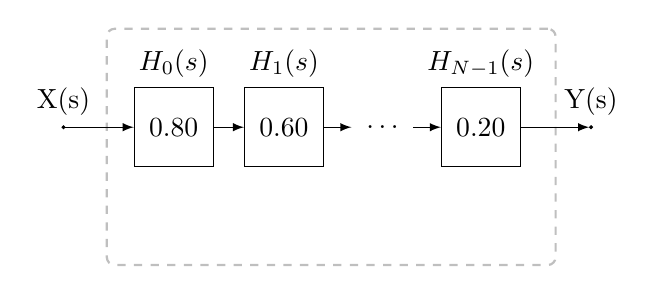
\begin{tikzpicture}
[scale=1, node distance=1.4cm, >=latex,
block/.style={
	rectangle, minimum size=10mm, minimum width=10mm, inner sep=2pt,
	draw=black},
largeblock/.style={
	rectangle, minimum size=8mm, minimum width=8mm, inner sep=3pt, thick,
	draw=gray!50, dashed, rounded corners=1mm},
dot/.style={
	circle, minimum size=1pt, inner sep=0pt,
	fill=black, draw=black}]

% coordinates
\coordinate (input) at (0, 0);
\coordinate [right of=input] (h0);
\coordinate [right of=h0] (h1);
\coordinate [right of=h1, node distance=2.5cm] (hN);
\coordinate [right of=h1, node distance=1.25cm] (dots);
\coordinate [right of=hN] (output);
\coordinate [right of=h0, node distance=2cm, yshift=-0.25cm] (cascade);

% input and output nodes
\node [dot, label={X(s)}] (In) at (input) {};
\node [dot, label={Y(s)}] (Out) at (output) {};

% cascade
\node [largeblock, minimum size=3cm, minimum width=5.7cm,
       label={[yshift=-2.85cm] \shelf}]
       (Cascade) at (cascade) {};

% biquads
\node [block, label={[yshift=0] $H_{0}(s)$}] (H0) at (h0) {\biquad{0.80}};
\node [block, label={[yshift=0] $H_{1}(s)$}] (H1) at (h1) {\biquad{0.60}};
\node [block, label={[yshift=0] $H_{N-1}(s)$}] (HN) at (hN) {\biquad{0.20}};


% signal flow
\draw [->] (In) -- (H0);
\draw [->] (H0) -- (H1) node [above, pos=0.5] {};
\draw [->] (H1.east) -- ++(0.35, 0) {};
\draw [<-] (HN.west) -- ++(-0.35, 0) {};
\draw [->] (HN) -- (Out) node [above, pos=0.5] {};
\node at (dots) {$\ldots$};

\end{tikzpicture}
\end{plottikz}

\end{document}

\caption{Signal flow for shelving filter cascade with input $X(s)$, output $Y(s)$ and
biquads $H_\mu(s)$ in series in the Laplace domain.}
\label{fig:tikz-cascade-biquads}
\end{subfigure}
%
\\\vspace{0.3cm}
%
\begin{subfigure}{0.45\textwidth}
\centering
\begin{plottikz}
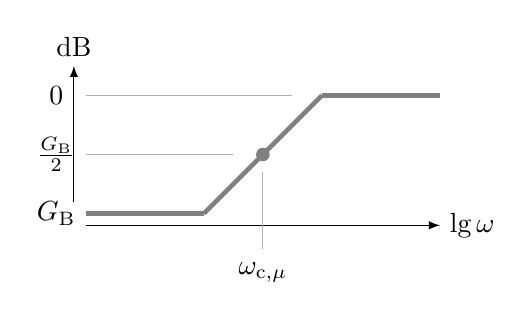
\begin{tikzpicture}[scale=1.5]
\draw [-latex] (0,-0.1) -- (3,-0.1) node [right]  {$\lg \omega$};
\draw [-latex] (-0.1,0.1) -- (-0.1,1.25) node [above]  {dB};
\draw [gray, ultra thick] (0,0) -- (1,0);
\draw [gray, ultra thick] (1,0) -- (2,1);
\draw [gray, ultra thick] (2,1) -- (3,1);
\draw[gray, fill=gray] (1.5,0.5) circle (1.5pt);
\node at (-0.25,1) {$0$};
\node at (-0.25,0.5) {$\frac{G_\mathrm{B}}{2}$};
\node at (-0.25,0) {$G_\mathrm{B}$};
\node at (1.5,-0.5) {$\omega_{\mathrm{c},\mu}$};
\node at (1,-0.25) {};
\node at (2,-0.25) {};
%
\draw [thin, black!30] (0,1) -- (1.75,1);
\draw [thin, black!30] (0,0.5) -- (1.25,0.5);
\draw [thin, black!30] (1.5,-0.3) -- (1.5,0.35);
%
\end{tikzpicture}
\end{plottikz}
\caption{Level response $20\lg |H_\mu(\omega)|$ of low-shelving
biquad for $G_\mathrm{B}<0$ and mid-level cutoff frequency $\omega_{\mathrm{c},\mu}$.
%The transition between the pass band and the shelving band can be somewhat controlled
%by $Q$, which then yields under-/overdamped responses.
}
\label{fig:schematic_magres_2nd_ls}
\end{subfigure}
%
\\\vspace{0.3cm}
%
\begin{subfigure}{0.45\textwidth}
\centering
\begin{plottikz}
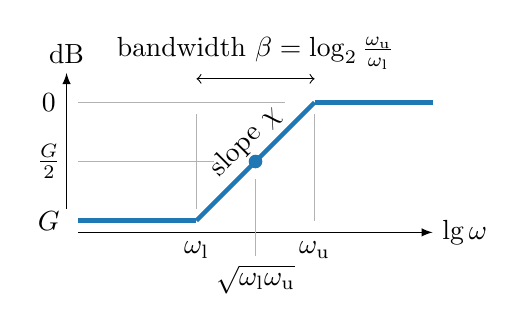
\begin{tikzpicture}[scale=1.5]
\draw [<->] (1,1.2) -- node [above] {bandwidth $\beta=\log_2{\frac{\omega_\mathrm{u}}{\omega_\mathrm{l}}}$}  (2,1.2) ;
\node [opacity=0] (first) {};
\node [draw=white, right of=first,rotate=45,anchor=north,xshift=1.5cm, yshift=0.2cm] {slope $\chi$};
%
\draw [-latex] (0,-0.1) -- (3,-0.1) node [right]  {$\lg \omega$};
\draw [-latex] (-0.1,0.1) -- (-0.1,1.25) node [above]  {dB};
\draw [color=pyplotC0, ultra thick] (0,0) -- (1,0);
\draw [color=pyplotC0, ultra thick] (1,0) -- (2,1);
\draw [color=pyplotC0, ultra thick] (2,1) -- (3,1);
\draw[color=pyplotC0, fill=pyplotC0] (1.5,0.5) circle (1.5pt);
\node at (-0.25,1) {$0$};
\node at (-0.25,0.5) {$\frac{G}{2}$};
\node at (-0.25,0) {$G$};
\node at (1.5,-0.5) {$\sqrt{\omega_\mathrm{l} \omega_\mathrm{u}}$};
\node at (1,-0.25) {$\omega_\mathrm{l}$};
\node at (2,-0.25) {$\omega_\mathrm{u}$};
%
\draw [thin, black!30] (0,1) -- (1.75,1);
\draw [thin, black!30] (0,0.5) -- (1.15,0.5);
\draw [thin, black!30] (1.5,-0.3) -- (1.5,0.35);
\draw [thin, black!30] (2,0) -- (2,0.9);
\draw [thin, black!30] (1,0.1) -- (1,0.9);
%
\end{tikzpicture}
\end{plottikz}
\caption{Level response $20\lg |H(\omega)|$ of shelving filter cascade
for $G<0$ and lower/upper cutoff frequency $\omega_\mathrm{l/u}$. For a dedicated
$\omega_\mathrm{u}$,
additionally two of the three parameters $\chi$, $\beta$ and $G$ can be freely
adjusted.}
\label{fig:schematic_magres_2nd_arb}
\end{subfigure}
%
\caption{Signal-flow graph (a) and schematic level responses of a single 2nd
order shelving filter (b) and the proposed shelving filter cascade (c).}
\label{fig:schematic_magres}
\end{figure}


\begin{figure*}[t]
\centering
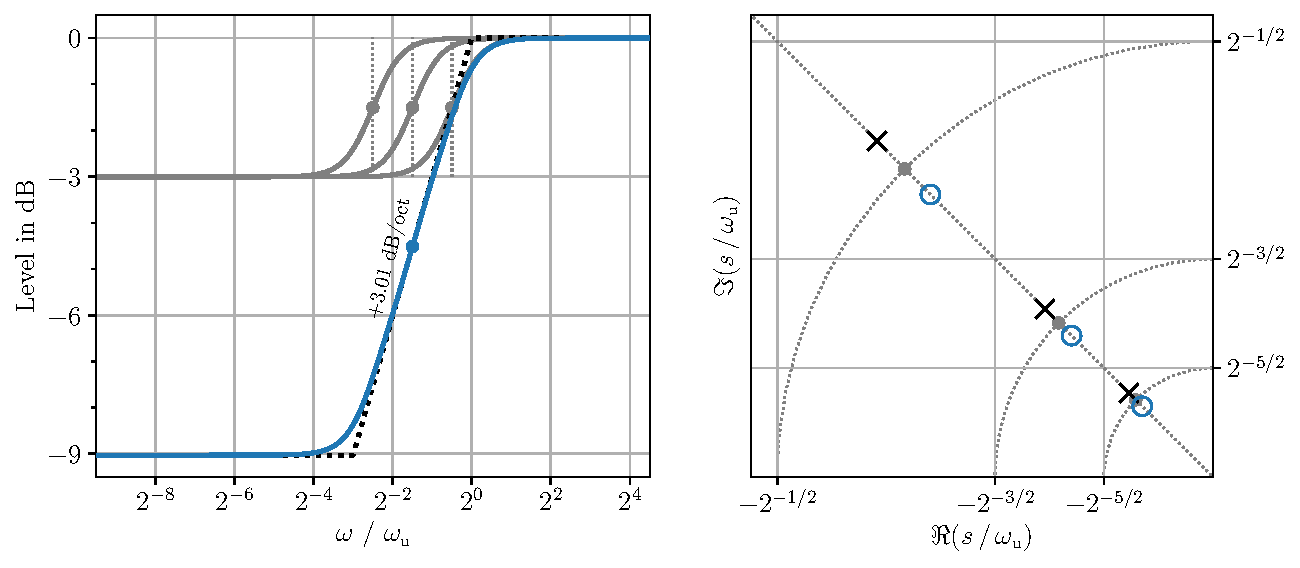
\includegraphics[width=0.8\textwidth]{../graphics/biquad-and-pzmap.pdf}
\caption{Left: Level responses of the cascade of three biquads $H_\mu(s)$
(gray) building $H(s)$ (blue)
with $G = - 30 \lg(2) \approx - 9.03$ dB, $\chi = 10 \lg(2) \approx +3.01$ dB/oct,
$\beta=3$ oct. Right: Corresponding poles/zeros in upper/left $s$-plane with
linear axes scaling. Note that the conjugate-complex poles and zeros are not
shown, cf. \fig{fig:pzmap}. Logarithmic equidistance of the poles and zeros
and alignment along the line which is determined by the $Q$-factor is fundamental for
the filter design.}
\label{fig:biquad-and-pzmap}
\end{figure*}

%
\subsection{Parameters}
%
Based on the fundamental diffusive representation
\cite[Sec. 3.2]{Helie2013},
the cascade \eq{eq:cascade} allows to build shelving filters with fractional-order slopes.
%
Particularly, the design of a shelving filter is possible, where two of the
three intended parameters (cf. \fig{fig:schematic_magres_2nd_arb})
%
\begin{itemize}
\setlength\itemsep{-0.1em}
\item $\chi\neq0$: transition slope in dB/oct
\item $\beta>0$: transition bandwidth in octaves
\item $G$: shelving level in dB
\end{itemize}
%
can be defined by the user, determining the third one from (signs: $-$ for low
shelving filter, $+$ for high shelving filter)
\begin{align}
\label{eq:parameter_triplet}
G = \mp\,\beta \cdot \chi,\qquad
\beta = \bigg|\frac{G}{\chi}\bigg|,\qquad
\chi = \mp\,\frac{G}{\beta}.
\end{align}
%
%
%
For the log-log human hearing characteristics (i.e. amplitude and
frequency resolution) \cite{Fastl2007},
it appears reasonable to equally space the individual mid-level cutoff
frequencies $\omega_{\mathrm{c},\mu}$ on a logarithmic frequency axis.
%
Thus, a user definable parameter is the number of cascaded biquads per
octave $N_{O}$.
%
%
%
%
%
%
\NewL The mid-level cutoff frequencies of the biquads in the cascade \eq{eq:cascade}
may then be stated as
%
\begin{align}
\omega_{\mathrm{c},\mu} = 2^{-(\mu+\frac{1}{2})/N_{O}} \cdot \omega_\mathrm{u}
\end{align}
%
with a user definable upper cutoff frequency $\omega_\mathrm{u}$ in rad/s of the
shelving filter cascade $H(s)$.
%
From the intended bandwidth $\beta$ the lower cutoff frequency of $H(s)$ reads
\begin{align}
\omega_\mathrm{l} = 2^{-\beta} \cdot \omega_\mathrm{u},
\end{align}
%
which can be rewritten to
\begin{align}
\beta = \log_2 \frac{\omega_\mathrm{u}}{\omega_\mathrm{l}}.
\end{align}
%
In \fig{fig:schematic_magres_2nd_arb} the level response
is schematically shown with the introduced variables.
%
The shelving level is equal for each biquad $H_\mu(s)$ and is given by
\begin{align}
\label{eq:Gb}
G_\mathrm{B} = - \frac{\chi}{N_{O}}
\end{align}
in dB.
%
For the user defineable number of biquads $N_O$ per octave,
the total number of required biquads
$N$ for the whole cascade is derived as
\begin{align}
\label{eq:ceil_function}
N = \lceil \beta \cdot N_{O} \rceil
\end{align}
with the ceiling operation $\lceil \cdot \rceil$ yielding nearest larger integer.
%
%
%
%
%
%
\section{Analog Filter Properties}
\label{sec:analog_filter_properties}
%
Other than typical shelving filters,
where shelving level determines the slope characteristics,
the proposed filter cascade allows for adjustable slope and bandwidth.
%
This is exemplarily demonstrated in the following.
%
All plots use the normalized frequency $\omega/\omega_\mathrm{u}$,
therefore the upper cutoff frequency of the shelving filter cascade
$\omega_\mathrm{u}$ needs no explicit definition.
%
%
%Note that increased $Q$ also increases
%
%Tuning of $Q$ is straightforward and behaves similar to traditional shelving
%filters.
%
%Thus, no further details are presented for this issue.
%
\subsection{Working Principle}
%
In \fig{fig:biquad-and-pzmap} the working principle of the filter is shown
with a cascade of $N=3$ biquads and $N_O=1$ biquad per octave.
%
The parameter triplet is chosen to
$G = - 30 \lg(2) \approx - 9.03$ dB,
$\chi = 10 \lg(2) \approx +3.01$ dB/oct
and $\beta=3$ oct.
%
According to \eq{eq:Gb}, the biquad shelving level is
$G_\mathrm{B} = -10 \lg(2) \approx -3.01$ dB.
%
Butterworth factor $Q=\nicefrac{1}{\sqrt{2}}$ \cite[p.792]{Ballou2008} is used.
%Butterworth factor $Q=\nicefrac{1}{\sqrt{2}}$ is used.
%
The Laplace transfer functions can be calculated with the formulas given in
Sec. \ref{sec:filter_design}.
%
The left plot of \fig{fig:biquad-and-pzmap} depicts the level responses of
the individual biquads (gray, cf. \fig{fig:schematic_magres_2nd_ls}),
of the shelving filter cascade (blue, cf. \fig{fig:schematic_magres_2nd_arb}),
and the ideal piecewise linear level response (dotted black line).
%
Due to chosen $N_O=1$, the mid-level cutoff frequencies $\omega_{\mathrm{c},\mu=0,1,2}$
are distributed by integer octaves.
%
The right plot in \fig{fig:biquad-and-pzmap} shows the poles and zeros
that lie in the upper-left $s$-plane.
%
In total, six poles and six zeros (three 2nd order sections each with a
conjugate-complex pole and zero pair) build the shelving filter cascade.
%
The gray dots indicate the mid-level frequencies
$|s_{\mathrm{c},\mu}|=\omega_{\mathrm{c},\mu}$ for $\mu=0,1,2$.
%
With help of the circles,
the values for $\omega_{\mathrm{c},\mu}$ can be read at $\Im(s)$-axis.
%
Furthermore, along the line intersecting all gray dots
(i.e. $\angle s = \nicefrac{3}{4}\pi$ for the chosen $Q=\nicefrac{1}{\sqrt{2}}$),
also all poles and zeros are aligned, cf.
\fig{fig:pzmap}.
%
This pole/zero alignment is typical and fundamental \cite{Helie2013}
for the proposed filter design, which is in contrast to the equiangular
alignment used in
\cite{Holters2006a}, see \fig{fig:holters2006-higher-order-shelving}.
%
%
%
\NewL The chosen $Q$-factor has impact on the achieved frequency response.
%
Around the cutoff frequencies, varying $Q$ has about the same impact as for a
single 2nd order shelving filter.
%
However, for the shelving filter cascade, varying $Q$ has an impact
on the slope and the bandwidth as well.
%
Generally, increasing $Q$ increases ripples along the slope in level and
phase.
%
Decreasing $Q$ decreases the bandwidth, where the intended slope holds.
%
Butterworth factor $Q=\nicefrac{1}{\sqrt{2}}$ and
$Q=\nicefrac{5}{6}$ \cite[p.261]{LangeSigSys1} are good
trade-off choices to obtain moderately damped responses at lower/upper
cutoff frequencies as well as small slope ripple and valid slope bandwidth.
%
To keep focus on other details, this issue is not further
discussed here and in the remainder all filters use Butterworth factor
$Q=\nicefrac{1}{\sqrt{2}}$.

\begin{figure*}
\centering
\begin{subfigure}{0.8\textwidth}
\centering
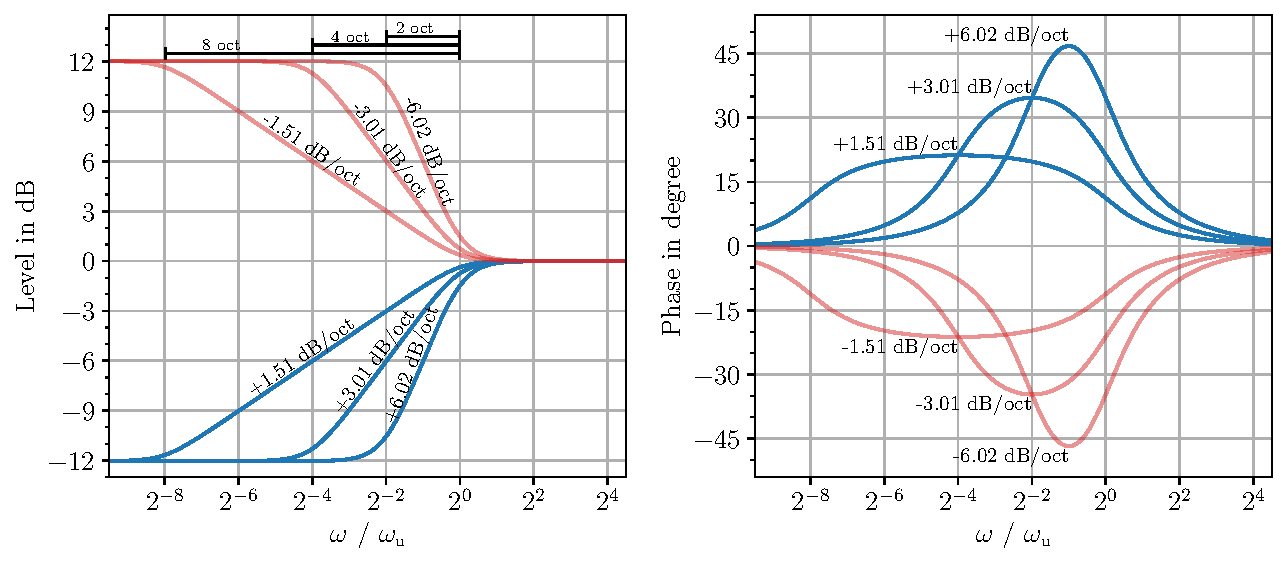
\includegraphics[width=\textwidth]{../graphics/low-shelving-filter-varying-slope.pdf}
\caption{Fixed shelving level $G=\pm 20 \lg (4) \approx \pm 12$ dB.
Varied slope $\chi$ in
dB/oct with resulting bandwidth $\beta$ in octaves or vice versa.}
\label{fig:low-shelving-filter-varying-slope}
\end{subfigure}
\\
\begin{subfigure}{0.8\textwidth}
\centering
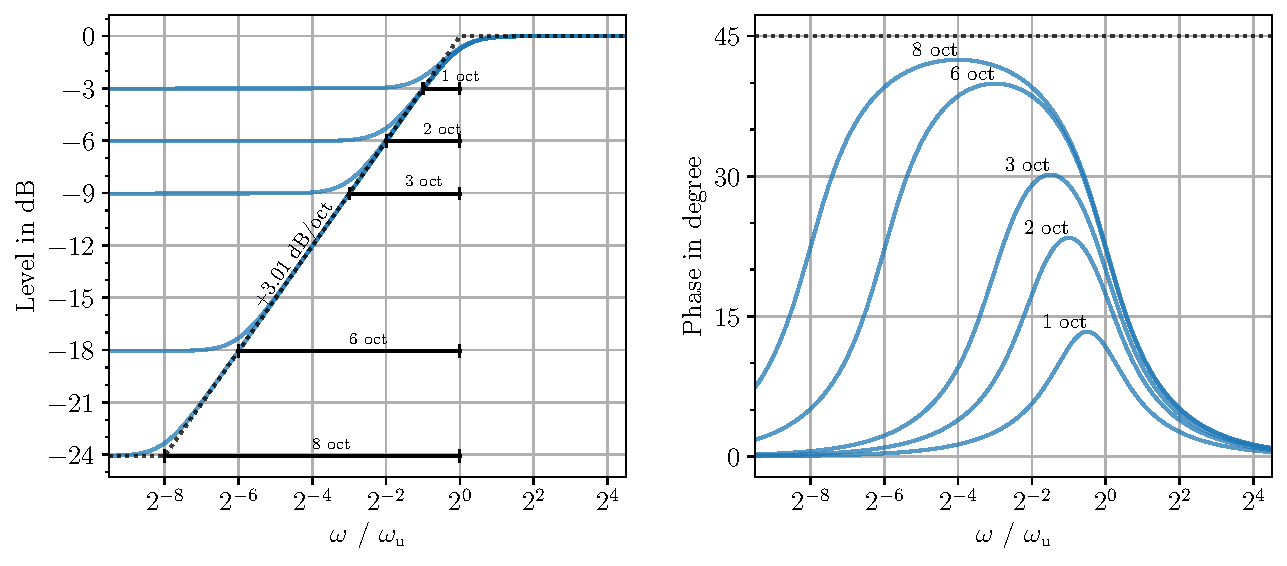
\includegraphics[width=\textwidth]{../graphics/low-shelving-filter-varying-bandwidth.pdf}
\caption{Fixed slope $\chi = 10\lg(2)\approx + 3.01$ dB/oct. Varied bandwidth
$\beta$ in octaves, resulting shelving level $G$ in dB or vice versa.}
\label{fig:low-shelving-filter-varying-bandwidth}
\end{subfigure}
\\
\begin{subfigure}{0.8\textwidth}
\centering
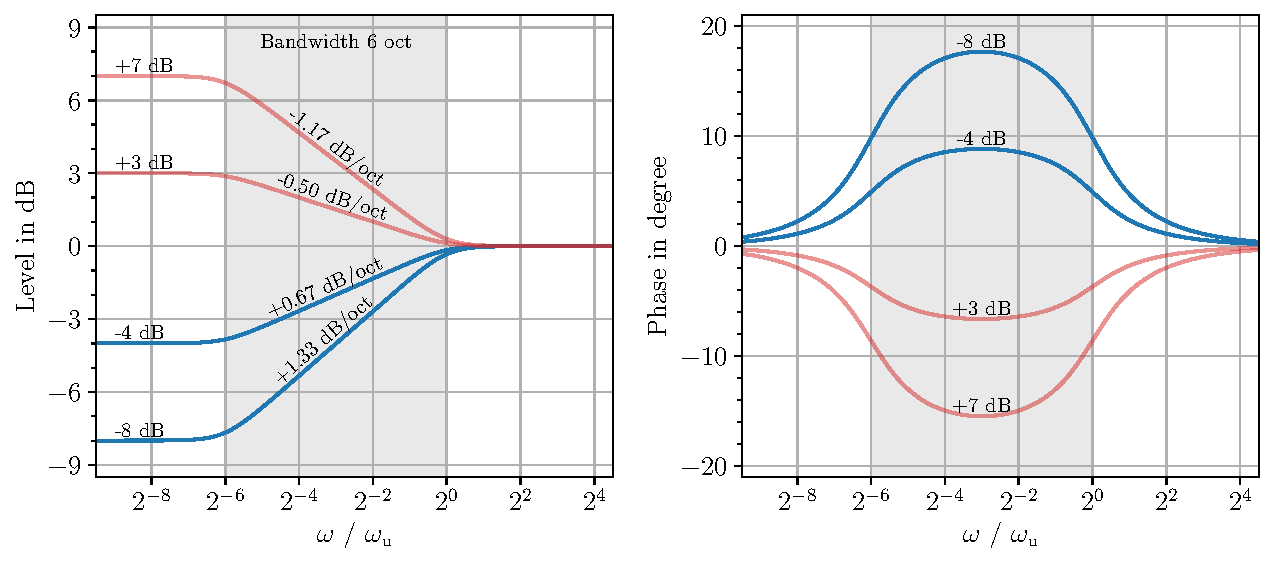
\includegraphics[width=\textwidth]{../graphics/low-shelving-filter-varying-gain.pdf}
\caption{Fixed bandwidth $\beta=6$ octaves. Varied shelving level $G$ in dB,
resulting slope $\chi$ in dB/octave or vice versa.}
\label{fig:low-shelving-filter-varying-gain}
\end{subfigure}
%
\caption{Shelving filter cascade frequency responses.
Two of the three design parameters $\chi$, $\beta$ and $G$
can be freely chosen, determining the third one. Depending on the target
application one of the three setup strategies might be preferable.}
\label{fig:shelving_filter_setup_cases}
\end{figure*}


\subsection{Frequency Responses}
%
In \fig{fig:shelving_filter_setup_cases} different variations of the
parameter triplet shall illustrate the capabilities of the shelving filter
cascade.
%
Each of the left plots shows the resulting level response in dB and each of
the right plots depicts the phase response in degree.
%
All filter cascades exhibit $N_O = 3$ biquads per octave.
All chosen bandwidths are integer values.
Then \eq{eq:ceil_function} yields the number of required biquads
$N = 3\cdot\beta$ and thus filter order $M=2 \cdot N=6\cdot\beta$,
which is convenient for mental calculation.
%
%
%
\NewL In \fig{fig:low-shelving-filter-varying-slope} the shelving level
$G=\pm 20 \lg (4) \approx \pm 12$ dB is fixed.
%
Then either slope $\chi$ or bandwidth $\beta$ can be additionally adjusted.
%
The slopes $\chi = \mp 10 \lg (\sqrt{2}, 2, 4) \approx \mp 1.5, 3, 6$
dB/oct are adjusted
yielding the bandwidths $\beta = 8,4,2$ octaves, respectively using \eq{eq:parameter_triplet}.
%
The somewhat laborious values for $\chi$ were used
because these represent exact
multiples of a first-order system slope of $\pm 20 \lg(2)$ dB/oct.
With chosen $G$ this then results in integer values
for $\beta$.
%
The depicted level responses in
\fig{fig:low-shelving-filter-varying-slope} verify the intended shelving
characteristics.
%
The phase responses indicate minimum-phase characteristics, with
the generally known observations, that phase excess becomes larger the steeper
the slope and the larger the shelving level.
%
For the particular filter with 8 octave bandwidth,
minimum-phase characteristics of constant $\pm22.5$ degrees for
$\chi = \pm 10 \lg\sqrt{2} \approx \pm 1.5$ dB/oct is approximated in a large
frequency band.
%
This is expected for a quarter-differentiator/-integrator.
%
%
%
\NewL In \fig{fig:low-shelving-filter-varying-bandwidth},
$\chi = 10\lg(2)\approx +3.01$ dB/oct is fixed.
%
A positive slope requires a negative shelving level, which can be chosen as
further adjustable parameter.
%
Alternatively, the bandwidth as free parameter can be adjusted, which is pursued
here with $\beta = 1,2,3,6,8$ octaves.
%
With \eq{eq:parameter_triplet} this yields shelving levels
$G = - 10\lg(2)\cdot (1,2,3,6,8)\approx -(3,6,9,18,24)$ dB.
%
The level responses clearly show the intended characteristics.
%
The phase response shows the increasing phase excess in value and frequency
bandwidth with increasing transition bandwidth.
%
The filter with 8 octaves bandwidth approximates $+45$ deg constant
minimum-phase (dotted line) for a large frequency band, resembling half-differentiator
filter characteristics (ideally: +3.01 dB/oct slope and 45 deg phase).
%
%
%
\NewL In \fig{fig:low-shelving-filter-varying-gain} the bandwidth $\beta = 6$
octaves is fixed.
%
Either the slope or the shelving level can be additionally adjusted.
%
Here the chosen integer levels $G = 7,3, -4,-8$ dB yield slopes
$\chi = -\nicefrac{7}{6}, -\nicefrac{3}{6}, +\nicefrac{4}{6}, +\nicefrac{8}{6}$
dB/oct, respectively.
%
The level responses depict the expected characteristics.
%
The phase responses exhibit similar characteristics varying in their
maximum phase excess, which is linked to the shelving level and the achieved
slope.
%
Thus, again: a certain fractional-order slope involves a certain minimum phase
(offset).
%
In the case of an ideal slope over the whole frequency band,
a constant phase
$\angle H(\omega) = \frac{\pi}{2} \frac{\chi}{20\lg(2) \mathrm{dB}/\mathrm{oct}}$
in radian results.
%


\subsection{Constraints and Limitations}
%
Naturally for approximations---in the present case a fractional-order
slope is approximated with a finite number of biquads and a certain octave
resolution---deviations to the ideal case are to be expected.
%
This subsection exemplarily discusses the general limitation patterns of the
proposed filter design method.
%
In \fig{fig:shelving_filter_error_cases} these limitations are
visualized.
%
In \fig{fig:gain-error} the effect of shelving level quantization is depicted.
%
Since the parameter triplet $G, \beta, \chi$ influences $N$ (which
needs to be integer) and $N_O$, only certain $\beta$ and $G$ can be exactly realized with
a chosen parameter set.
%
Note that $\omega_\mathrm{u}$ can be completely freely adjusted though.
%
From \eq{eq:Gb}, \eq{eq:ceil_function}, the resulting shelving
level $G_\mathrm{r}$ thus reads
\begin{align}
G_\mathrm{r} = G_\mathrm{B} \cdot N  = - \frac{\chi}{N_{O}} \cdot
\lceil \beta \cdot N_{O} \rceil
\end{align}
for chosen $\chi$, $\beta$ and $N_O$.
%
Only for $\beta \cdot N_{O}\in\mathbb{N}$ the intended shelving level is equal to
the resulting level $G_\mathrm{r} = G$.
%
The larger the deviation $\beta \cdot N_{O}$ towards the next larger integer,
the larger is the quantization error for the shelving level.
%
This can be reproduced with the chosen parametrization in \fig{fig:gain-error}
for slope
$\chi = +10\lg(2) \approx +3.01$ dB/oct,
bandwidth $\beta=\nicefrac{19}{6}$ octaves and shelving level
$G= - \chi \cdot \beta \approx - 9.53$ dB.
%
Only $N_O = 6$ biquads per octave yield integer $\beta \cdot N_{O} = 19$
and thus $G_\mathrm{r} = G$.
%
This quantization effect must be considered in practical designs and
a tolerable, application dependent quantization step size must be defined by the
user.
%
\NewL In \fig{fig:slope-error} it is demonstrated that the desired slope and
bandwidth is not always being achieved when the chosen parameters are set
unfavorable.
%
The intended bandwidth and slope is well approached if both rule-of-thumb
conditions
\begin{align}
\label{eq:bchiNO_cond}
&\beta \cdot N_O \in \mathbb{N}\\\nonumber
&N_O \geq
\begin{cases}
\frac{\chi}{12\,\mathrm{dB}} &\,\,\,\mathrm{if}\,\,\,\chi \geq 12 \, \mathrm{dB/oct}\\
1 / \mathrm{oct} &\,\,\,\mathrm{if}\,\,\,\chi < 12 \, \mathrm{dB/oct}
\end{cases}
\end{align}
are met at the same time, following from
maximum slope of 12 dB/oct for a 2nd order filter.
%
For \fig{fig:slope-error} the parameter triplet
$\chi = +120 \lg(2) \approx +36$ dB/oct, $\beta = 3$ oct,
$G = -360 \lg(2) \approx -108$ dB was set up.
%
For the chosen $N_O = \nicefrac{1}{3}, \nicefrac{2}{3}, 1, 3$
the first condition of \eq{eq:bchiNO_cond}
always holds, which also yields $G_\mathrm{r}=G$, see discussion for \fig{fig:gain-error}.
%
However, only $N_O=3$ fulfills the second condition of \eq{eq:bchiNO_cond},
then the resulting slope and bandwidth converge well to the intended one.
%
For the other cases the bandwidth appears to be larger.
%
In the extreme case of $N_O=1/3$ only one biquad is utilized, due to
$N = \lceil \beta \cdot N_{O} \rceil$.
%
This single biquad obviously cannot render the
intended frequency response, but rather exhibits that of a
2nd order shelving filter.
%
\begin{figure*}
\centering
\begin{subfigure}{0.8\textwidth}
\centering
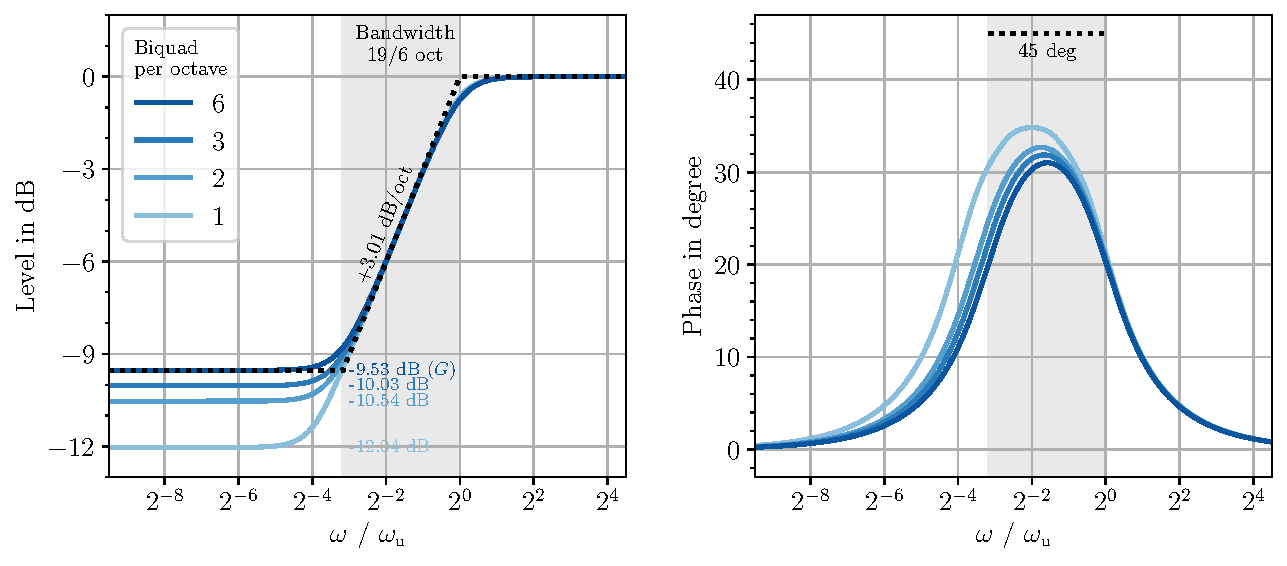
\includegraphics[width=\textwidth]{../graphics/gain-error.pdf}
\caption{Slope $\chi = 10\lg(2)\approx +3.01$ dB/oct and shelving
level $G=-\frac{19}{6} \cdot \mathrm{oct} \, \chi \approx - 9.53$ dB yields a bandwidth
of $\beta = 19/6$ octaves.
The resulting shelving level deviates from $G$ for less than $N_O = 6$
biquads per octave.}
\label{fig:gain-error}
\end{subfigure}
\\
\begin{subfigure}{0.8\textwidth}
\centering
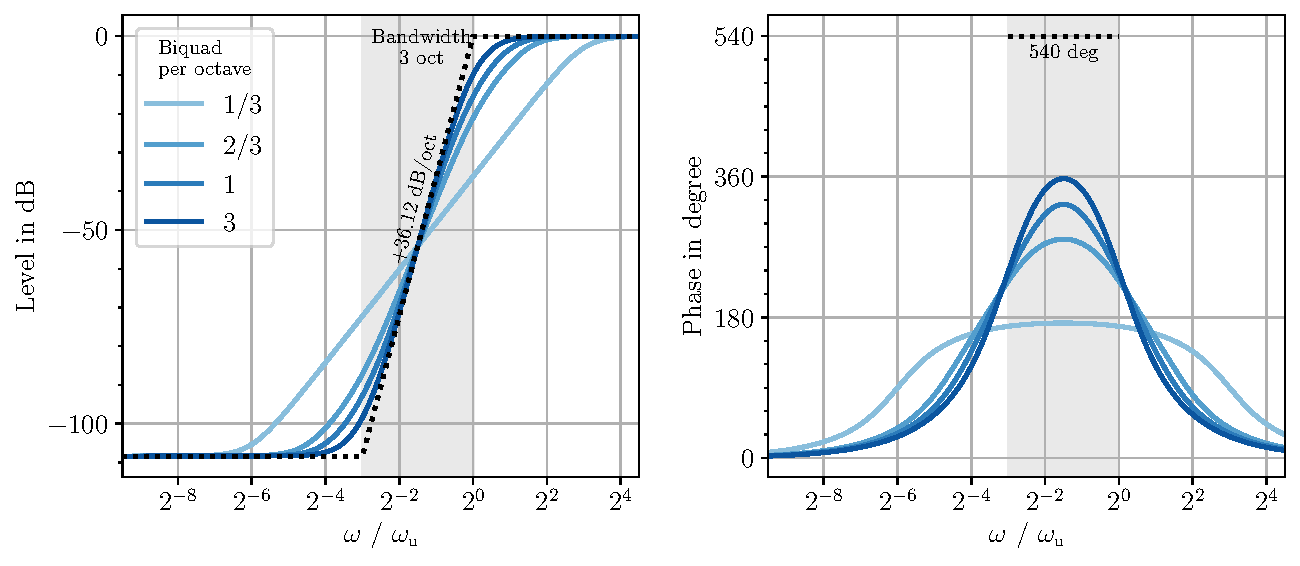
\includegraphics[width=\textwidth]{../graphics/slope-error.pdf}
\caption{Slope $\chi = 120 \lg(2) \approx +36\,\mathrm{dB/oct}$ and bandwidth $\beta=3$
octaves yields shelving level $G=-360\lg10(2) \approx -108$ dB.
The resulting bandwidth deviates from $\beta$ when deploying less than $N_O = 3$
biquads per octave.
}
\label{fig:slope-error}
\end{subfigure}
\\
\begin{subfigure}{0.8\textwidth}
\centering
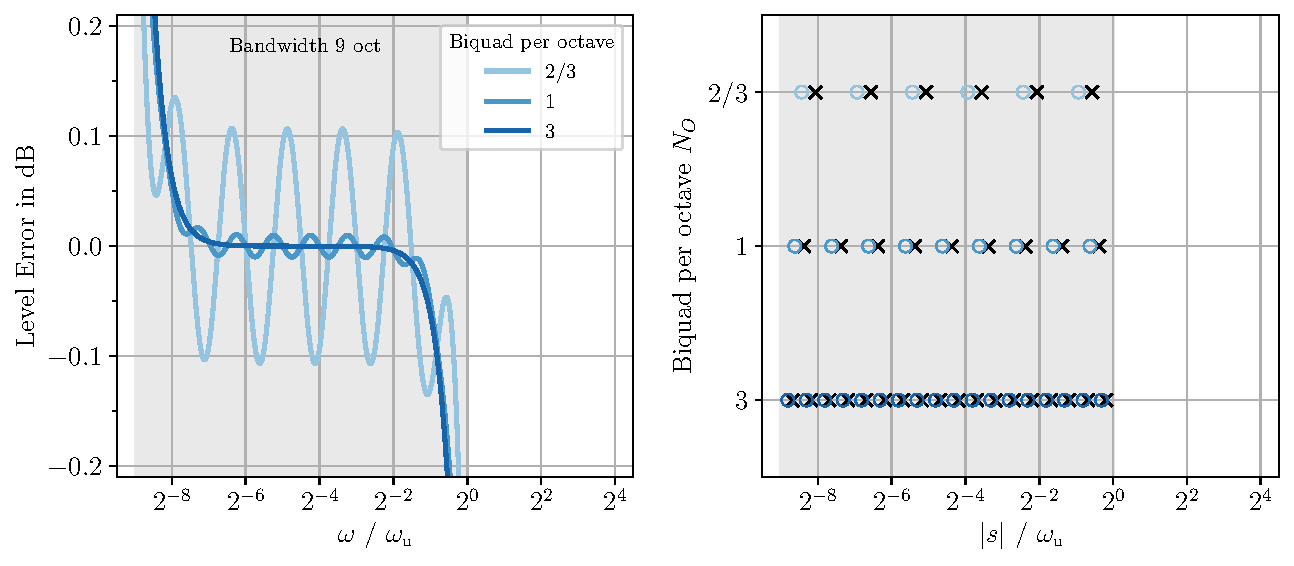
\includegraphics[width=\textwidth]{../graphics/ripple-and-zp-frequency.pdf}
\caption{$\beta=9$ oct,
$G=-10\lg(2)\approx -3$ dB yields
$\chi =  \frac{10}{9}\lg(2) \approx + 0.3345$ dB/oct.
Left: $20\lg|H(\omega)|-20\lg|H_\mathrm{ideal\,slope}(\omega)|$.
Right: distribution of poles (x) and zeros (o).}
%depending on number of biquads
%per octave.
\label{fig:ripple-and-zp-frequency}
\end{subfigure}
%
\caption{Shelving filter cascade frequency responses.
%
Limitations of the filter design method occur due to the discrete number of
cascaded biquads to represent a fractional-order filter slope.
}
\label{fig:shelving_filter_error_cases}
\end{figure*}

%
\begin{figure*}[t]
\centering
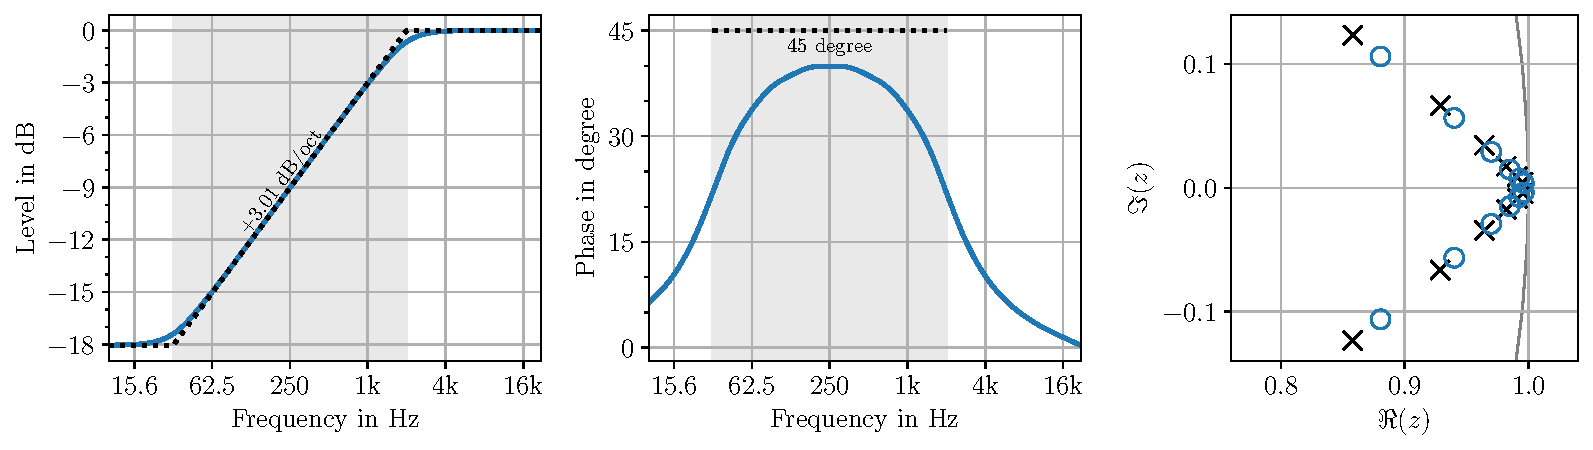
\includegraphics[width=\textwidth]{../graphics/digital-3db-per-octave-shelving-filter.pdf}
\caption{
Digital shelving filter cascade with bilinear $z$-transform for
$\chi = 10\lg(2) \approx 3.01$ dB/oct and bandwidth $\beta=6$ octaves, upper
cutoff frequency 2 kHz, sampling frequency 48 kHz, $N_O=1$ biquad per oct.
%
Left: level response, middle: phase response, right: poles/zeros in
$z$-plane.
}
\label{fig:digital-3db-per-octave-shelving-filter}
\end{figure*}
%
\NewL In \fig{fig:ripple-and-zp-frequency} the case of slope ripple as a
function of biquads per octave is discussed.
%
As stated above, the fractional slope is approximated by biquads that are
spaced with certain fractional-octave resolution.
%
Thus it is expected, additionally to the already mentioned limitations,
that the slope exhibits ripples in the level response.
%
For \fig{fig:ripple-and-zp-frequency} the parameter triplet
$\beta=9$ oct,
$G=-10\lg(2)\approx -3$ dB,
$\chi =  \frac{10}{9}\lg(2) \approx + 0.3345$ dB/oct
is set up, realized with
$N_O = \nicefrac{2}{3}, 1, 3$.
%
The condition $\beta \cdot N_O\in\mathbb{N}$ is always fulfilled, thus $G_\mathrm{r}=G$.
%
The choice $N_O=\nicefrac{2}{3}$ violates the 2nd condition of \eq{eq:bchiNO_cond},
whereas $N_O=1,3$ fulfill it.
%
The deviation with respect
to the ideal piecewise linear slope (cf. \fig{fig:schematic_magres_2nd_arb})
is visualized in terms of the error
$20\lg|H(\omega)|-20\lg|H_\mathrm{ideal\,slope}(\omega)|$.
%
It can be clearly observed as a rippled slope response.
%
For $N_O = \nicefrac{2}{3}$ biquads per octave the ripple amounts $\pm 0.1$ dB.
%
For $N_O=3$ biquads per octave the ripple becomes irrelevantly small for
practical audio applications.
%
Note that the error steeply increases at the edges of the transition band,
since the resulting filter naturally deviates from the ideal piecewise linear
slope.
%
Again, one can state that the suitable amount of biquads per octave is highly
dependent on the tolerated ripple.
%
One biquad per octave resolution seems to be a good trade-off for most
audio applications that ask for slopes $|\chi|<12$ dB/oct.
%
%
\NewL In summary, all three limitations and generally $\beta\gg 1$ octave (which in
practice can be relaxed to $\beta>1$),
must be taken into account by the filter designer to customize towards a target
application.

%The proposed design requires more biquads than traditional designs and thus
%more computational load, which nowadays should be acceptable.
%
%Rippe increase for Q incresae!!

\begin{figure}[h!]
\centering
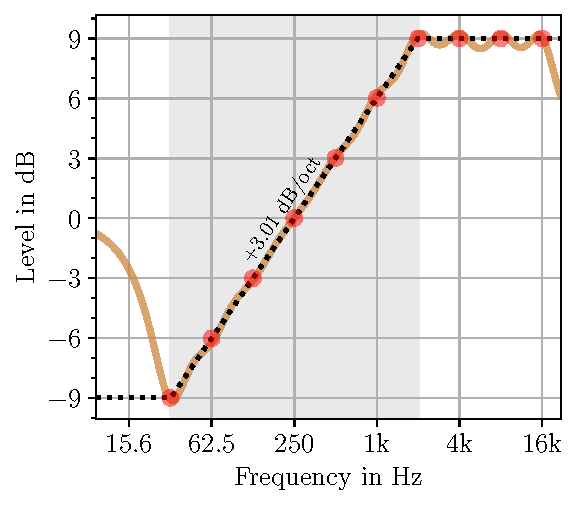
\includegraphics[width=0.68\columnwidth]{../graphics/liski2019-geq-3db-per-oct.pdf}
\caption{Digital GEQ \cite{Liski2019} with $f_\mathrm{s}=48$ kHz. The same shelving slope and bandwidth as in
\fig{fig:digital-3db-per-octave-shelving-filter} is intended by setting the
faders (red dots) accordingly.
GEQ has one octave resolution to be comparable with
\fig{fig:digital-3db-per-octave-shelving-filter}}
\label{fig:liski2019-geq-3db-per-oct}
\end{figure}








\section{Discussion}
\label{sec:discussion}
%
In this section some notes on digital filter design are given.
%
Furthermore, a comparison to a recent cascade GEQ design is presented
and potential meaningful applications are briefly outlined.

\subsection{Digital Filter Design}
\label{sec:digital_filter}
%
So far, analog filter responses were discussed.
%
For practical applications digital filters might be conveniently deployed
instead.
%
Digital filter design is straightforward with either the bilinear or the
matched $z$-transform of the individual 2nd order
analog filters \cite{Ifeachor2002,Berners2003,Nielsen2016}
or as Regalia-Mitra structure with a digital allpass \cite{Jot2015}.
%
If the upper cutoff frequency $f_\mathrm{u} = \frac{\omega_\mathrm{u}}{2\pi}$ is low
compared to the sampling frequency $f_\mathrm{s}$, the introduced artifacts are negligible.
%
In fact, for $f_\mathrm{u} / f_\mathrm{s} < \frac{1}{3}$ appropriate results are yielded,
spanning almost the whole listening range for typical audio sampling frequencies.
%
In \fig{fig:digital-3db-per-octave-shelving-filter} a digital shelving filter
with 6 octave bandwidth and 3 dB/oct slope is depicted for
$f_\mathrm{u}=2$ kHz and $f_\mathrm{s}=48$ kHz using bilinear transform without
frequency pre-warping.
%
For this example the matched z-transform practically yields the same results.
%
Both digital filters closely match the analog target response.
%
%
%
%\NewL Note that (standard) finite impulse response (FIR) designs exhibit a linear
%frequency scale.
%
%A similar shelving filter designed as FIR would require a rather long impulse
%response to achieve the frequency resolution in the low end.
%
%Thus, the number of biquads in IIR design and the number of taps in FIR design
%should be thoroughly evaluated for practical realizations.

\subsection{Comparison to Graphical Equalizer Design}
%
GEQs can be used to approach a shelving filter characteristic with
certain slope over certain bandwidth.
%
In \fig{fig:liski2019-geq-3db-per-oct} this is exemplarily shown, deploying
a very recently proposed GEQ design by Liski \cite{Liski2019}.
%
The filter shall have +3.01 dB/oct slope within 6 octave bandwidth with upper
cutoff frequency of 2 kHz, i.e. the same as
\fig{fig:digital-3db-per-octave-shelving-filter}.
%
The GEQ is designed from a PEQ cascade, which inherently
makes constant level over a larger bandwidth an ambitious task.
%
Thus, compared to the shelving filter cascade, the ripple at the 9 dB constant
level band is larger and the -9 dB level band is not realized at all.
%
Furthermore, a slightly larger ripple along the slope can be observed for the
GEQ by close inspection.
%
Although, the resulting filter might be acceptable, setup of different slopes
and bandwidth in a GEQ might be tedious.
%
Thus, if explicitly requiring shelving filter characteristics,
the proposed shelving filter
cascade could be preferred with its simpler parameter set and more accurate response.

\subsection{Potential Applications}
%
The presented filter could be used in audio mixing and production,
where transition bandwidth might be an additional
parameter for shelving filters.
%
The proposed filter design might improve the loudness filter of \cite{Nielsen2016},
where a cascade of two 1st order shelving filters was designed to compensate
for equal loudness level contours.
%
The dual-band shelving filter
approach \cite{Audfray2018} could make use of the proposed filter.
%
%
%
\NewL Usually bass boosted target transfer functions are desired for large-scale
sound reinforcement, which can be conveniently realized with the proposed
filter design.
%
Furthermore, also so called line \textit{array morphing}
\cite{LAcoustics2013} can be approached with either varying the
shelving level and the slope (\fig{fig:low-shelving-filter-varying-slope})
or varying the level and the bandwidth (\fig{fig:low-shelving-filter-varying-gain}).
%
%
%
\NewL As another example, for wave field synthesis (WFS) \cite{Firtha2017} and
line source array (LSA) applications, a shelving filter
with a +3 dB/oct rising slope, ideally with +45 degree phase,
for the mid-frequency band is required
in order to equalize the inherent acoustic lowpass characteristic of the
deployed line source.
%
The proposed filter design can be straightforwardly parametrized to obtain this
commonly known WFS pre-filter and LSA coupling filter.
%
The frequency responses shown in
\fig{fig:low-shelving-filter-varying-bandwidth} and
\fig{fig:digital-3db-per-octave-shelving-filter}
are typical examples for it.
%
The lower shelf compensates for the loudspeaker array's omni-directional
characteristic at lower frequencies, where array length determines the lower
cutoff frequency \cite{Schultz2016}.
%
The upper shelf compensates for spatial aliasing energy \cite{Spors2010a}, here
upper cutoff frequency is varied to match the different spatial aliasing cutoff
frequencies of sound field synthesis (SFS) methods \cite{Winter2018}.
%
Furthermore, dynamically changing the filter parameters is straightforward and
could be advantageously deployed for dynamic SFS, such as WFS of moving
sources \cite{Firtha2019}.
%
For SFS of focused point sources, filter responses with two different
(fractional-order) slopes are required \cite{Spors2010,Spors2011}.
%
This could be realized with an optimized shelving filter cascade that exhibits
multiple slopes.
%
%
%
\NewL Multiple slope filters, or more generally multiband EQ design is out of
scope of this paper.
%
However, the band-shelving filter concept of \cite{Holters2006a} can be
straightforwardly adopted for our filter design, which then could enhance the
control of the transition bands with adjustable slope and bandwidth.



\section{Summary}
\label{sec:summary}
%
This paper proposes a cascade of second-order shelving filters to realize a
higher-order shelving filter with adjustable transition slope and adjustable
transition bandwidth additionally to the common parameters cutoff frequency
and shelving level.
%
As a natural choice regarding human hearing, the mid-level frequencies of the
biquads are equidistantly aligned with respect to logarithmic frequency axis.
%
Thus, a critical parameter is the number of biquads per octave, which must be
sufficiently high to achieve the intended frequency response, most important
a ripple free shelving slope.
%
Digital filter design for audio applications can be straightforwardly realized
with bilinear or matched-z transform of individual biquads.
%
This IIR filter based design might be preferably used for specific
applications rather than specialized FIR designs or GEQs.
%
With its simple parametrization, the filter could be deployed in various
audio applications. %and to design parametric multiband EQs.


\begin{figure*}[h]
\centering
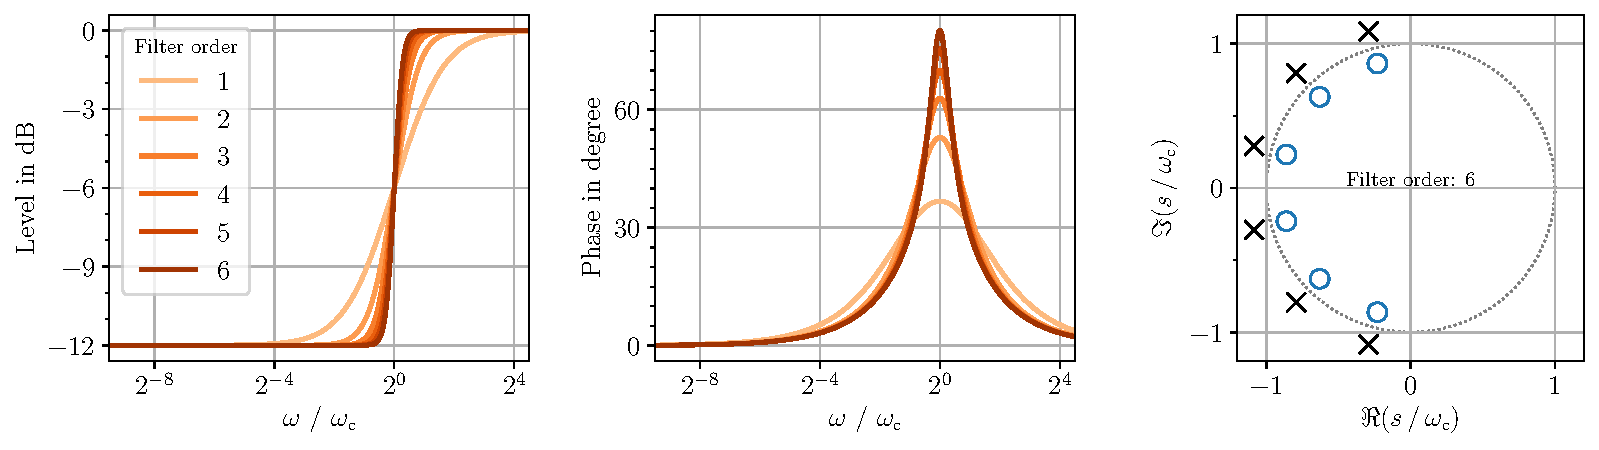
\includegraphics[width=\textwidth]{../graphics/holters2006-higher-order-shelving.pdf}
\caption{Higher order low-shelving filters from Holters \cite{Holters2006a}
adapted to $\omega_\mathrm{c}$ as mid-level cutoff frequency.
%
Then, poles and zeros are equiangularly aligned along the circle with radius
$|s| = \omega_\mathrm{c}$.
%
The larger the filter order the closer the poles and zeros are aligned to that
circle, cf. 2nd order filter pole/zero-map in \fig{fig:pzmap}.
%
An increasing slope and phase excess can be observed for increased filter order,
however no explicit control of transition bandwidth is possible.}
\label{fig:holters2006-higher-order-shelving}
\end{figure*}




\section*{Appendix: Laplace Transfer Function of Traditional Shelving Filters}
%
The transfer function of a general 2nd order filter for real signals
reads
%
\begin{align}
\label{eq:generalHbiquad}
\tilde{H}(s) = \frac{b_2 s^2 + b_1 s + b_0}{a_2 s^2 + a_1 s + a_0}
\end{align}
for Laplace domain $s = \sigma + \im \omega$ with $b, a\in\mathbb{R}$.
%
For $s = \im \omega$ the frequency response
$\tilde{H}(\omega)=|\tilde{H}(\omega)|\e^{\im \angle \tilde{H}(\omega)}$ over angular
frequency $\omega$ is evaluated.
%
%
%
\NewL
The shelving filter is parametrized with
shelving level $G_\mathrm{B}$ in dB,
mid-level cutoff frequency $\omega_c$ in rad/s
and---for the 2nd order filter---the pole/zero $Q\geq\frac{1}{2}$ factor
(the same $Q$ for pole and zero is applied here for convenience).
%
With $g_\mathrm{B} = 10^{|G_\mathrm{B}| / 20}>0$ the coefficients for 1st/2nd
order low-/high-shelving
filters can be given in the following listing, cf. \cite{Spors2019}.
%
The $\pm$ exponent for $g_\mathrm{B}$ corresponds to the sign of $G_\mathrm{B}$,
i.e. positive or negative shelving level $G_\mathrm{B}$.
%
%
%
\NewL
%
The 1st order low-shelving filter is given by the coefficients
for \eq{eq:generalHbiquad}
\begin{align}
b_2 = 0,\quad b_1 = \frac{1}{\omega_\mathrm{c}},\quad b_0 = g_\mathrm{B}^{\pm\frac{1}{2}},\\\nonumber
a_2 = 0,\quad a_1 = \frac{1}{\omega_\mathrm{c}},\quad a_0 = g_\mathrm{B}^{\mp\frac{1}{2}}.
\end{align}
%
The 1st order high-shelving filter is given by
\begin{align}
b_2 = 0,\quad b_1 = \frac{g_\mathrm{B}^{\pm\frac{1}{2}}}{\omega_\mathrm{c}},\quad b_0 = 1,\\\nonumber
a_2 = 0,\quad a_1 = \frac{g_\mathrm{B}^{\mp\frac{1}{2}}}{\omega_\mathrm{c}},\quad a_0 = 1.
\end{align}
%
The 2nd order low-shelving filter is given by the
coefficients for \eq{eq:generalHbiquad}, cf. \cite[(15)]{Valimaki2016}
\begin{align}
\label{eq:LS2nd}
b_2 = \frac{1}{\omega_\mathrm{c}^2},\quad b_1 = \frac{g_\mathrm{B}^{\pm\frac{1}{4}}}{Q\,\omega_\mathrm{c}},\quad b_0 = g_\mathrm{B}^{\pm\frac{1}{2}},\\\nonumber
a_2 = \frac{1}{\omega_\mathrm{c}^2},\quad a_1 = \frac{g_\mathrm{B}^{\mp\frac{1}{4}}}{Q\,\omega_\mathrm{c}},\quad a_0 = g_\mathrm{B}^{\mp\frac{1}{2}}.
\end{align}
%
The 2nd order high-shelving filter is given by
\begin{align}
b_2 = \frac{g_\mathrm{B}^{\pm\frac{1}{2}}}{\omega_\mathrm{c}^2},\quad b_1 = \frac{g_\mathrm{B}^{\pm\frac{1}{4}}}{Q\,\omega_\mathrm{c}},\quad b_0 = 1,\\\nonumber
a_2 = \frac{g_\mathrm{B}^{\mp\frac{1}{2}}}{\omega_\mathrm{c}^2},\quad a_1 = \frac{g_\mathrm{B}^{\mp\frac{1}{4}}}{Q\,\omega_\mathrm{c}},\quad a_0 = 1.
\end{align}
%
\definecolor{pyplotC0}{RGB}{31,119,180}
\begin{figure}[b!]
\centering
\begin{plottikz}
\begin{tikzpicture}[scale=1.8]
%
\draw[fill=gray!10,->,>=stealth] (0,0) -- (0:0.25) arc (0:135:0.25);
\node at (0.1,0.1) {$\alpha$};
%
\draw [-latex, thick] (-1.75,0) -- (0.5,0) node [right]  {$\Re(\frac{s}{\omega_\mathrm{c}})$};
\draw [-latex, thick] (0,-1.25) -- (0,1.25) node [above] {$\Im(\frac{s}{\omega_\mathrm{c}})$};
%
\draw[gray, dashed] (-1,1) -- (-1,-1);
\draw[gray, dashed] (-0.7071,0.7071) -- (-0.7071,0);
\draw[gray, dashed] (-0.5,0.5) -- (-0.5,-0.5);
\draw[gray, dashed] (-1,1) -- (0,1);
\draw[gray, dashed] (-0.5,0.5) -- (0,0.5);
\draw[gray, dashed] (-1,-1) -- (0,-1);
\draw[gray, dashed] (-0.5,-0.5) -- (0,-0.5);
\draw[gray, dashed] (-0.7071,0.7071) -- (0.15,0.7071);
%
\draw[gray, -latex] (-1,1) arc (135:150:1.4142);
\draw[gray, -latex] (-1,1) arc (135:120:1.4142);
\node at (-1.2,0.6) {$Q\downarrow$};
\node at (-0.55,1.25) {$Q\uparrow$};
%
\draw[gray, -latex] (-1,-1) arc (-135:-120:1.4142);
\draw[gray, -latex] (-1,-1) arc (-135:-150:1.4142);
\node at (-1.2,-0.6) {$Q\downarrow$};
\node at (-0.55,-1.25) {$Q\uparrow$};
%
%\draw[dashed] (-1.4142,-1.4142) -- (-1.4142,-0.5) node [left, above] {$-\sigma_0$};
%\draw[dashed] (-1.4142,+1.4142) -- (0,+1.4142) node [right] {$+\omega_D$};
%\draw[dashed] (-1.4142,-1.4142) -- (0,-1.4142) node [right] {$-\omega_D$};
%\node at (1.9,1) {$\omega_D = \omega_0 \sqrt{1-D^2}$};
%\node at (1.3,0.5) {$\sigma_0 = D \omega_0$};
%\node at (-0.7,0.25) {$\alpha$};
\node at (-1.1,-0.15) {-1};
\node at (-0.7071,-0.175) {$\frac{-1}{\sqrt{2}}$};
\node at (-0.4,-0.15) {$\frac{-1}{2}$};
\node at (0.1,1) {1};
\node at (0.15,-1) {-1};
\node at (0.3,0.7071) {$\frac{1}{\sqrt{2}}$};
\node at (0.1, 0.5) {$\frac{1}{2}$};
%
\node at (-1.2,1) {$s_\infty$};
\node at (-0.3,0.43) {$s_0$};
%
\draw[ultra thin, gray] (0,1) arc (90:270:1);
%
\draw[gray,fill=gray] (-0.7071,0.7071) circle (1.5pt);
%
\draw[gray, dashed] (0,0) -- node[pos=1, right] {}(+135:1.4142) node[solid, fill=white, cross=6pt, draw=black, ultra thick] {};
\draw[gray, dashed] (0,0) -- node[pos=1, right] {}(-135:1.4142) node[solid, fill=white, cross=6pt, draw=black, ultra thick] {};
\draw[gray, dashed] (0,0) -- node[pos=1, right] {}(+135:0.7071) node[solid, fill=white, circle, draw=pyplotC0, ultra thick] {};
\draw[gray, dashed] (0,0) -- node[pos=1, right] {}(-135:0.7071) node[solid, fill=white, circle, draw=pyplotC0, ultra thick] {};
%
\end{tikzpicture}
\end{plottikz}
\caption{Pole-zero map of 2nd order low-shelving filter with
shelving level $G_\mathrm{B} = - 20 \lg(4)$ dB and $Q=\nicefrac{1}{\sqrt{2}}$.
%
The mid-level cut-frequency $\omega_\mathrm{c}$ is represented as modulus of the gray
dot $\sqrt{|s_\infty| |s_0|}$.
%
Shifting poles and zeros along the lines away from $|s|=\omega_\mathrm{c}$ yields
$g_\mathrm{B}\uparrow$.
Shifting poles and zeros towards $|s|=\omega_\mathrm{c}$ yields $g_\mathrm{B}\to 1$.
%
Poles and zeros are reversed for positive shelving level $G_\mathrm{B}>0$ dB.
%
The damping characteristic is controlled by rotating all poles and zeros
around origin by $\alpha$.
}
\label{fig:pzmap}
\end{figure}

%
The 2nd order filter can be further discussed with the pole-zero map shown
in \fig{fig:pzmap}.
%
%\section*{Appendix II: Zeros and Poles}
%
The zeros and poles of a 2nd order low-shelving filter are
\begin{align}
s_{0} = \omega_\mathrm{c} \:g_\mathrm{B}^{\pm\frac{1}{4}} \: \e^{\im\alpha}\qquad
s_{\infty} = \omega_\mathrm{c} \: g_\mathrm{B}^{\mp\frac{1}{4}} \: \e^{\im\alpha},
\end{align}
and the respective complex conjugates $s_{0}^{\ast}$ and $s_{\infty}^{\ast}$.
The sign in the exponents is again determined
by the shelving level $G_\mathrm{B}$.
The polar angle $\alpha$ in the complex $s$-plane (Laplace domain)
relates to the $Q$-factor
\begin{align}
Q = \frac{-1}{2\cos\alpha}.
\end{align}
For stable and causal filters,
the poles must be in the left-half $s$-plane $\Re(s_{\infty}) < 0$,
hence requiring $\frac{\pi}{2} < \alpha < \frac{3\pi}{2}$.
The corresponding $Q$-factor is always positive
and varies within $[\frac{1}{2}, \infty)$.
This paper mainly considers Butterworth \cite{Ballou2008} $Q=\frac{1}{\sqrt{2}}$,
which yields $\alpha=\frac{3}{4} \pi$
as illustrated in Fig.~\ref{fig:pzmap}.
If $Q=\frac{1}{2}$, i.e. $\alpha=\pi$,
the poles and zeros lie on the real axis,
thus double real poles $s_{0} = s_{0}^{\ast}$ and
$s_{\infty} = s_{\infty}^{\ast}$ are obtained.
%
In this case the 2nd order frequency
response is identical to that of the 1st order shelving filter, although
obtained by different pole/zero-configurations.
%
Thus, it is sufficient to discuss the present filter design based on
2nd order filters.
%
\NewL In the case of high-shelving filters, the poles and zeros are exchanged. %,
%\begin{align}
%s_{0} &= \omega_{c,\mu} \: g_\mathrm{B}^{\mp\frac{1}{4}} \: e^{i\alpha}\\
%s_{\infty} &= \omega_{c,\mu} \: g_\mathrm{B}^{\pm\frac{1}{4}} \: e^{i\alpha}.
%\end{align}
Notice that a high-shelving filter with a shelving gain $\pm g_\mathrm{B}$
has the same poles and zeros as the low-shelving filter with $\mp g_\mathrm{B}$.
The system functions only differ by a scaling factor of $\pm g_\mathrm{B}$
due to the leading coefficients $b_{2}$ and $a_{2}$.
%
The scaling factor is lost information in a pole-zero map, unless explicitly
stated.
%
%
%%\section*{Appendix II: Zeros and Poles}
%
The zeros and poles of a 2nd order low-shelving filter are
\begin{align}
s_{0} = \omega_\mathrm{c} \:g_\mathrm{B}^{\pm\frac{1}{4}} \: \e^{\im\alpha}\qquad
s_{\infty} = \omega_\mathrm{c} \: g_\mathrm{B}^{\mp\frac{1}{4}} \: \e^{\im\alpha},
\end{align}
and the respective complex conjugates $s_{0}^{\ast}$ and $s_{\infty}^{\ast}$.
The sign in the exponents is again determined
by the shelving level $G_\mathrm{B}$.
The polar angle $\alpha$ in the complex $s$-plane (Laplace domain)
relates to
\begin{align}
Q = \frac{-1}{2\cos\alpha}.
\end{align}
For stable and causal filters,
the poles must be in the left-half $s$-plane $\Re(s_{\infty}) < 0$,
therefore $\frac{\pi}{2} < \alpha < \frac{3\pi}{2}$.
The corresponding $Q$-factor is always positive
and varies within $[\frac{1}{2}, \infty)$.
This paper mainly considers Butterworth \cite{Ballou2008} $Q=\frac{1}{\sqrt{2}}$
which leads to $\alpha=\frac{3}{4} \pi$
as illustrated in Fig.~\ref{fig:pzmap}.
If $Q=\frac{1}{2}$, i.e. $\alpha=\pi$,
the poles and zeros lie on the real axis,
thus double real poles $s_{0} = s_{0}^{\ast}$ and
$s_{\infty} = s_{\infty}^{\ast}$ are obtained.
%
In this case the 2nd order frequency
response is identical to that of the 1st order shelving filter, although
obtained by different pole/zero-configurations.
%
Thus, it is sufficient to discuss the present filter design based on
2nd order filters
%
\NewL In the case of high-shelving filters, the poles and zeros are exchanged. %,
%\begin{align}
%s_{0} &= \omega_{c,\mu} \: g_\mathrm{B}^{\mp\frac{1}{4}} \: e^{i\alpha}\\
%s_{\infty} &= \omega_{c,\mu} \: g_\mathrm{B}^{\pm\frac{1}{4}} \: e^{i\alpha}.
%\end{align}
Notice that a high-shelving filter with a shelving gain $\pm g_\mathrm{B}$
has the same poles and zeros as the low-shelving filter with $\mp g_\mathrm{B}$.
The system functions only differ by a scaling factor of $\pm g_\mathrm{B}$
due to the leading coefficients $b_{2}$ and $a_{2}$.

